\documentclass{article}

\usepackage[margin=1.5cm, includefoot, footskip=30pt]{geometry}

\usepackage{mathtools}
\usepackage{amsmath}
\usepackage{booktabs}
\usepackage{graphicx}
\usepackage{wrapfig}
\usepackage{caption}

\usepackage{biblatex}
\addbibresource{thesis.bib}

\title{An elementary analysis of the health board data}
\author{Henry Wilde}

\begin{document}
\maketitle




\section{Introduction}\label{sec:intro}

The contents of this document forms a basis for much of the data analysis and
mining techniques to come in the writing of this thesis. The data itself is
provided by the cwm taf university health board and is comprised of patient
records from across several nhs trusts in south wales.\\

As of December 2017, the dataset contains 2,447,475 patient records described by
259 attributes. These attributes are a mix of categorical, numerical, binary and
datetime variables that include: personal identifiers like age and gender; cost
components; clinical variables like current diagnoses, severity of diagnoses,
treatment site, length of stay, and procedures undertaken.\\

This analysis is themed largely on costs as this is the primary focus of the
thesis. As such, many of the plots will be against cost components or attributes
known to have a strong correlation with cost of treatment like length of stay.
However, before any analysis is done, it is important to understand the data we
are dealing with. In this section, we will define the attributes which describe
the dataset, as well as how the data has been cleaned to make it relatively
uniform. 


\subsection{Attributes}\label{subsec:attributes}

Of the 259 attributes, 104 of them are indicators of the presence of numerous
conditions as well as Charlson index scores to measure the severity of a
comorbidity. As there are several thousand different primary diagnoses present, 
belonging to roughly one thousand HRGs, and no immediate way of grouping those
together in a sensible way, we will not be considering any comparative analysis
between conditions or procedures except for those documented in the existing
literature.\\

The remaining 155 attributes are made up of roughly 30 attributes for various
component costs of treating a patient (ward costs, imaging, critical care,
etc.), and the rest are either personal identifiers (age, gender, ID numbers) or
more general clinical attributes such as start and end wards, length of stay,
treatment site, consultant, registered GP practice, or admission method. These
are the attributes we will focus this elementary analysis on.


\subsection{Formatting the data}\label{subsec:formatting}

After receiving the dataset, a substantial amount of preprocessing was done to
make certain attributes - and groups of attributes - consistent, as well as
removing a number of extra attributes which were added after data collection
that provided no additional information.\\


\section{Summative statistics}\label{sec:summative}

As was discussed in Section~\ref{subsec:attributes}, a large proportion of the 
attributes will not be considered in this analysis due to the volume of values 
the attributes take. However, cost components and non-specific clinical 
attributes are of interest.\\

When looking at this subset of attributes we can see that the data is heavily 
skewed toward short-stay, low-cost episodes and spells. The probability
density functions for length of stay and net cost are illustrated in Figures 
\ref{fig:LOS-kde}~\&~\ref{fig:NetCost-kde}, respectively, and show the extreme
nature of this skewedness.\\

\begin{figure}[h]
	\centering
	\begin{minipage}{.5\textwidth}
		\centering
		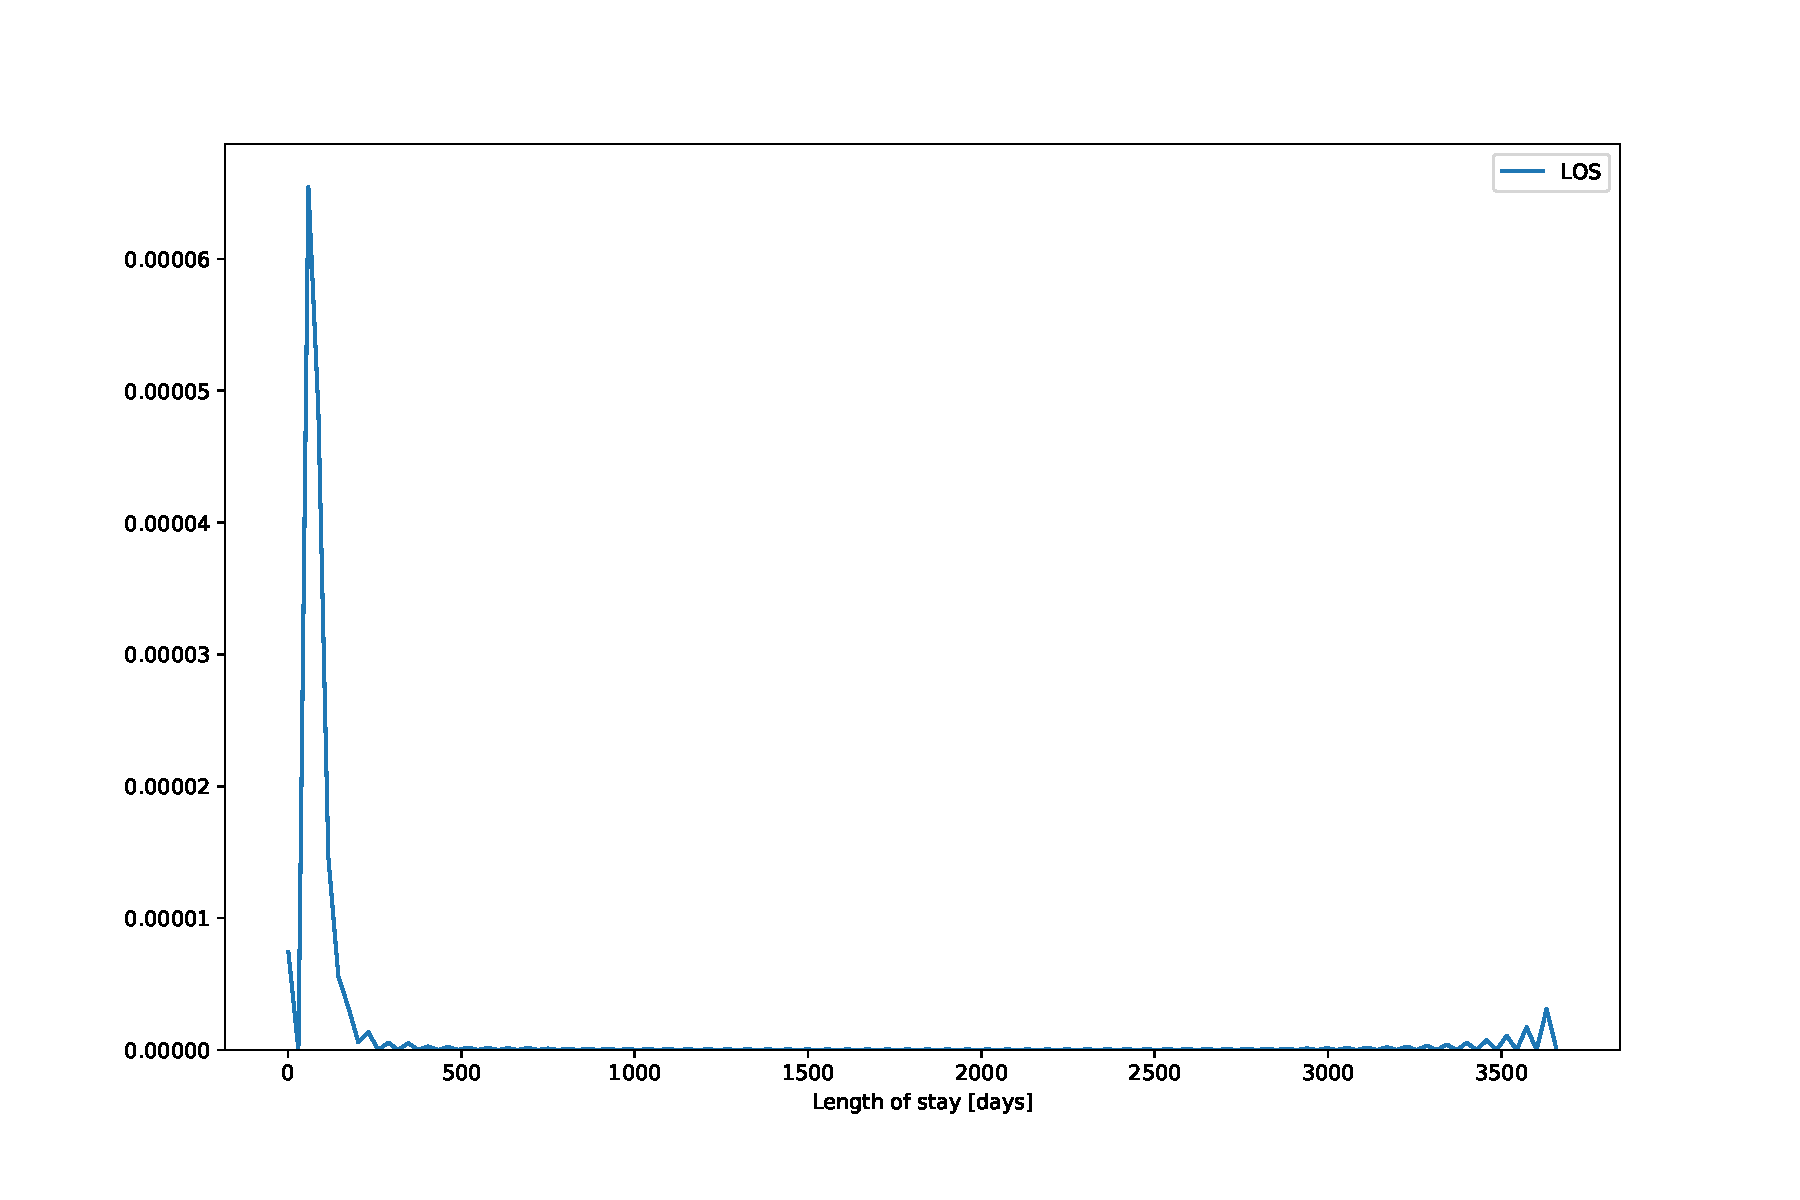
\includegraphics[width=\linewidth]{./img/LOS-kde.pdf}
		\captionof{figure}{Estimated p.d.f. for length of stay.}
		\label{fig:LOS-kde}
	\end{minipage}%
	\begin{minipage}{.5\textwidth}
		\centering
		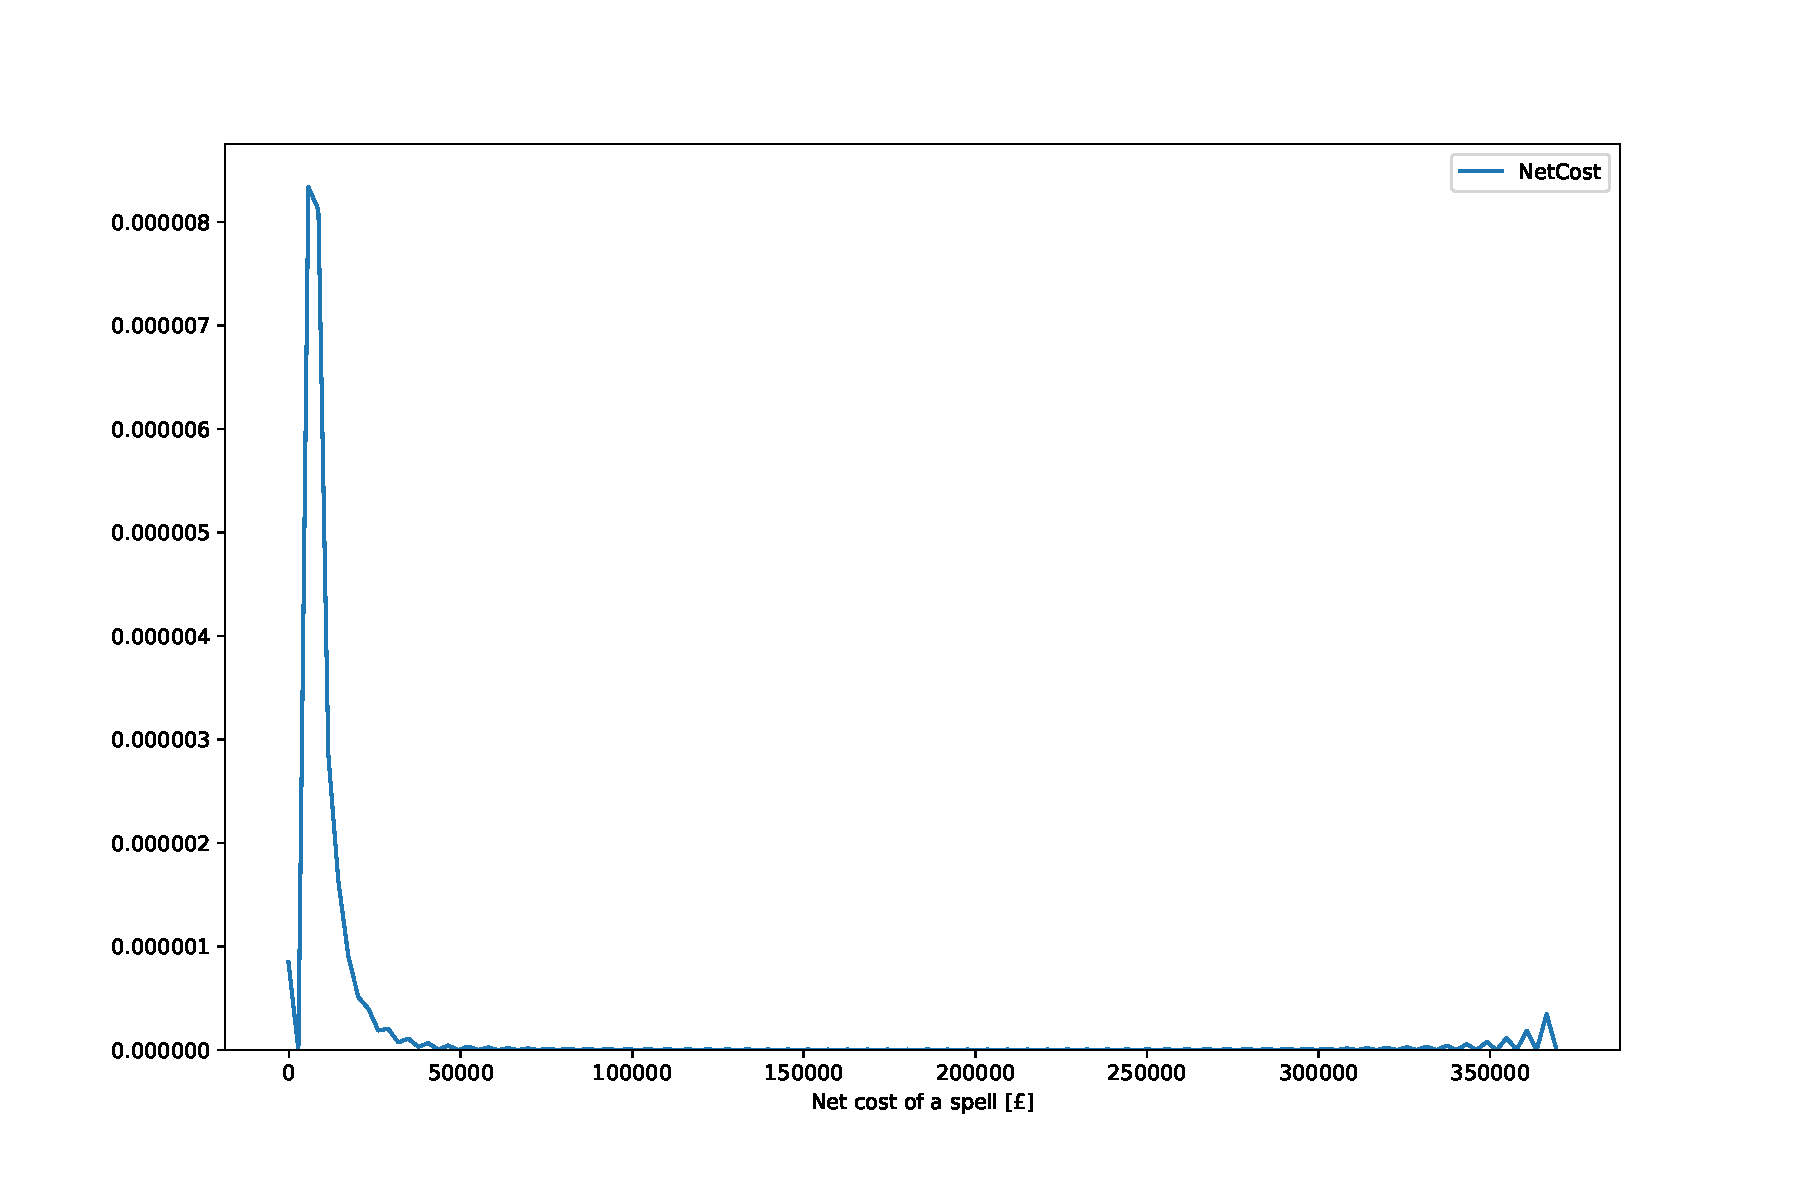
\includegraphics[width=\linewidth]{img/NetCost-kde.pdf}
		\captionof{figure}{Estimated p.d.f. for net cost.}
		\label{fig:NetCost-kde}
	\end{minipage}
    \begin{minipage}{.5\textwidth}
        \centering
        \includegraphics[width=\linewidth]{img/DIAG_NO-kde.pdf}
        \captionof{figure}{Estimated p.d.f. for number of diagnoses}
        \label{fig:DIAG_NO-kde}
    \end{minipage}%
    \begin{minipage}{.5\textwidth}
	    \centering
	    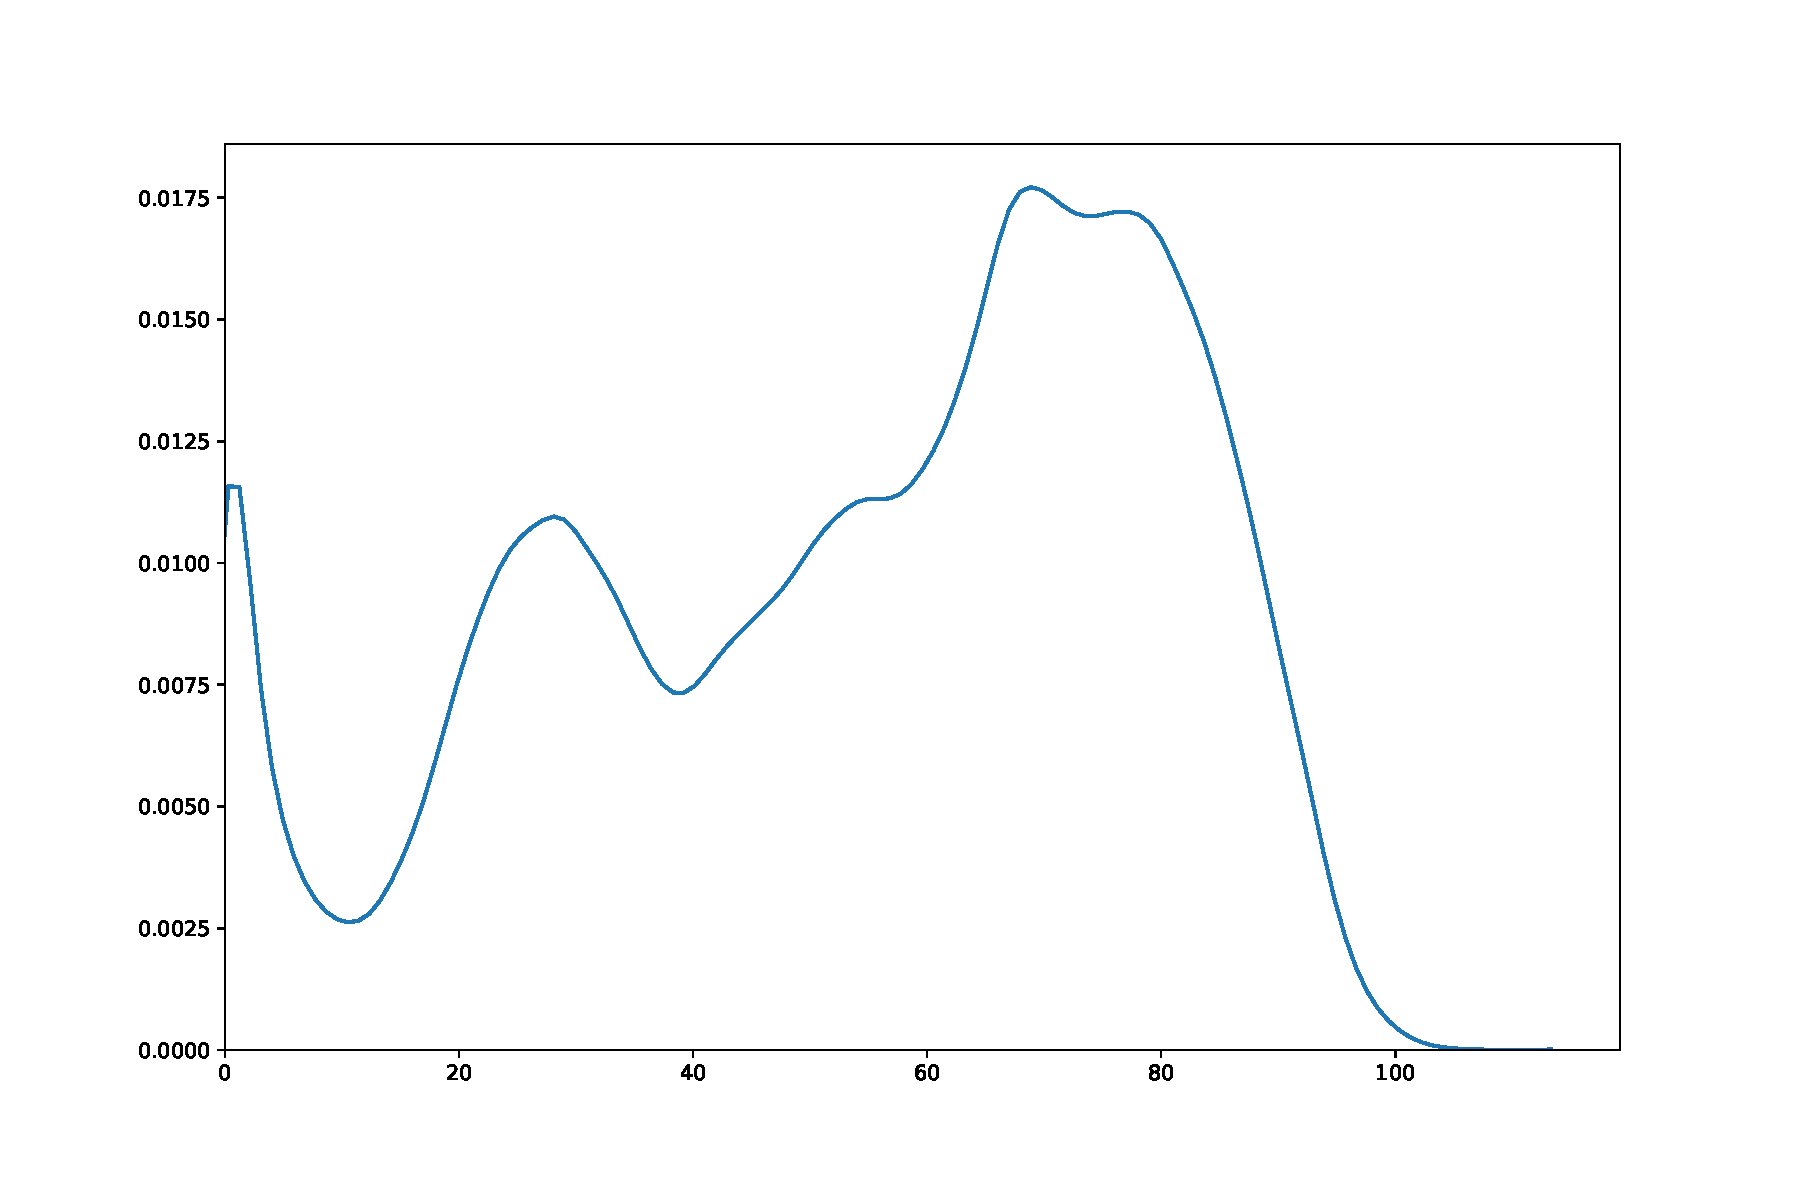
\includegraphics[width=\linewidth]{img/Age-kde.pdf}
	    \caption{Estimated p.d.f. for age.}
	    \label{fig:Age-kde}
    \end{minipage}
\end{figure}

This skewedness could be tackled either by means of scaling the data or some
other transformation of certain attributes, but that is not to say that 
all the attributes are so harshly skewed; Figure~\ref{fig:Age-kde} shows the
estimated p.d.f.\ for the age of a patient which has several very clear peaks 
and troughs.\\

\begin{figure}[h]
	\centering
	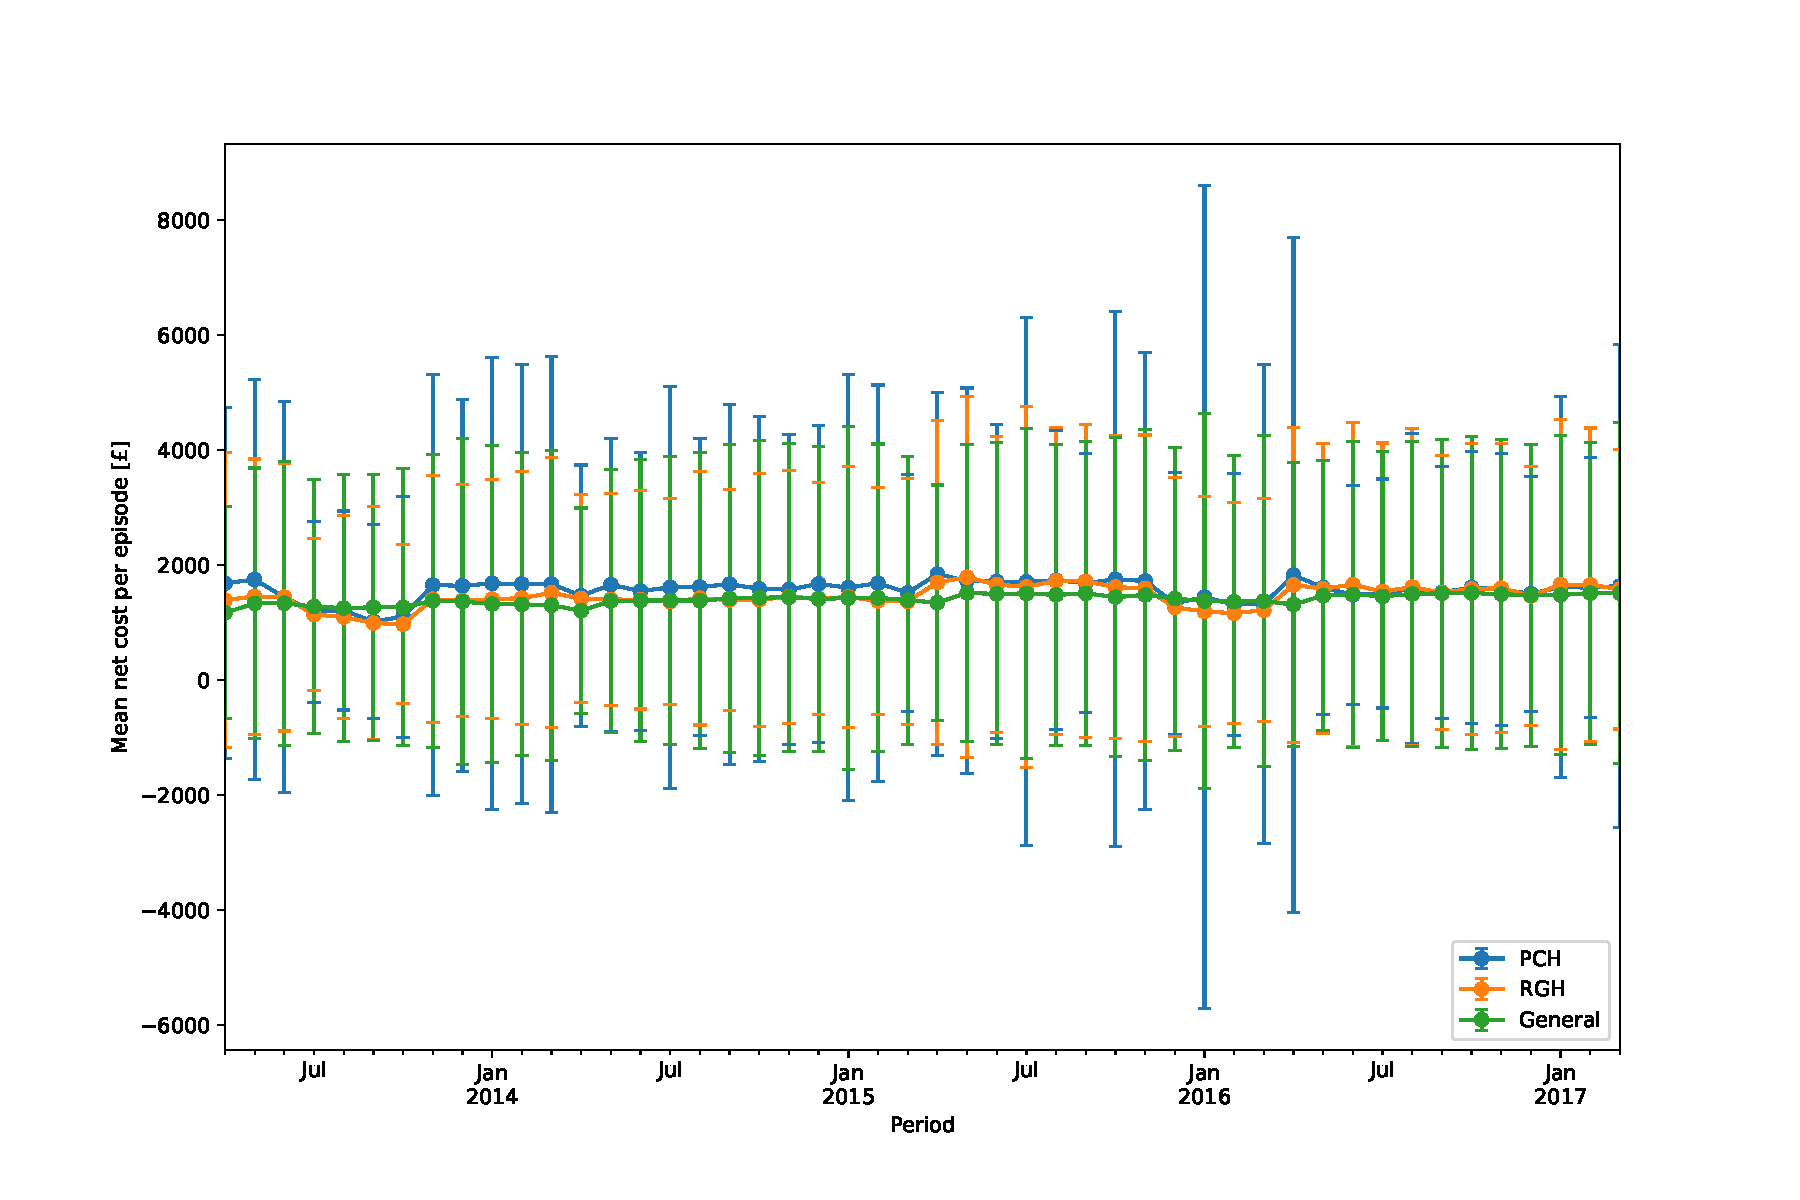
\includegraphics[width=.5\linewidth]{img/Mean-NetCost-by-site.pdf}
	\caption{A violin plot of the net cost of a spell, split across Prince 
        Charles Hospital, Royal Gwent Hospital and all records, including those
        without a specific treatment site.}
    \label{fig:mean-cost-by-site}
\end{figure}


\subsection{Summative statistics of selected attributes}\label{subsec:summative}

Refer to Table~\ref{tab:stats} for some basic statistics describing the 
attributes selected above. Note that, again, we can see the skewedness of our 
data by examining the sudden increase in values across the interquartile 
range.\\

This is not wholely surprising given that, in an anecdotal way, we would expect 
the `average' patient in a given NHS system will be there for a short period of 
time with some smaller (and probably less expensive) condition. The larger and 
more extreme values likely come from the cost of scheduled, expert work or more 
elongated forms of care.

\begin{table}[h]
	\resizebox{\textwidth}{!}{%
	\begin{tabular}{l|c|c|c|c|c|c|c|c|c|c|c|c|c|c}
		{} & Age & Length of stay & No. procedures & No. diagnoses & 
		Net cost & Critical care & Medical & Ward & Blood & Pathology &
		Prosthetics & Imaging & Pharmacy & Overheads \\ 
		\hline
		Mean & 53.956 & 3.514 & 1.894 & 4.921 & 1742.39 & 92.30 & 346.95 
		& 497.04 & 2.06 & 36.23 & 40.66 & 32.69 & 30.48 & 354.79 \\
		\hline
		Std. dev. & 25.835 & 8.646 & 2.203 & 6.897 & 3181.09 & 1335.04 &
		740.13 & 1234.45 & 37.17 & 135.61 & 343.35 & 143.52 & 86.70 & 
		732.58 \\
		\hline
		Min. & 0 & 1 & 0 & 0 & 4.5 & 0 & 0 & 0 & 0 & 0 & 0 & 0 & 0 & 0 
		\\ 
		\hline
		25\% & 33 & 1 & 0 & 1 & 347.52 & 0 & 44.45 & 10.33 & 0 & 0 & 0 &
		0 & 2.26 & 84.86 \\ 
		\hline
		50\% & 59 & 1 & 1 & 3 & 747.39 & 0 & 130.67 & 142.22 & 0 & 4.67 
		& 0 & 0.08 & 7.26 & 139.61 \\ 
		\hline
		75\% & 75 & 2 & 3 & 6 & 1863.95 & 0 & 375.08 & 463.95 & 0.15 & 
		31.93 & 0 & 10.93 & 26.29 & 321.76 \\ 
		\hline
		Max. & 109 & 3659 & 58 & 455 & 369168.90 & 250000.60 & 116449.90
		& 203854.10 & 13768.71 & 70008.12 & 68029.58 & 46708.66 & 25087.73 & 
        10428.60 \\
	\end{tabular}
	}
	\caption{Summative statistics for some of our cost components
	as well as other numerical attributes. Costs (\textsterling), lengths of
	stay (days) and numbers of procedure/diagnoses are all per spell.}
	\label{tab:stats}
\end{table}


\subsection{Correlation between attributes}\label{subsec:corr-cov}

Figure~\ref{fig:corr-heatmap} shows the Pearson correlation coefficient of all 
pairs of our selected attributes (not including age) in the form of a heatmap.
Representing data in this way is much easier to read and gain insight from than
trying to study a table of numbers.

\begin{figure}[h]
    \centering
    \includegraphics[width=.75\textwidth]{img/corr-heatmap.pdf}
    \caption{A heatmap of correlation coefficients for our cost components, and
        some other clinical attributes}
    \label{fig:corr-heatmap}
\end{figure}

There are several attributes, such as Secondary Comissioning Costs (SECC), that 
have no significant linear correlation with any of the other attributes but it 
is worth noting that there are clear correlations between many of the 
attributes; some of these are easier to realise than others. For instance, the 
longer the patient stays in a hospital, the longer they will likely be on the 
ward. This is why we see a strong positive correlation between ward costs and 
length of stay. Similarly, the longer a patient is on a ward for, the more 
overheads (like meals and administrative processes) they incur.

\section{Known areas of interests}\label{sec:known}

Given the amount of literature available around the following sections as well
as the works previously completed by the health board, we should attempt to
understand how the attributes associated with them settle in the data.

\subsection{Diabetes}\label{subsec:diabetes}

Can we see immediately what separates patients with diabetes (primary or
secondary) from those without? Do clusters exist in costs for those with and
without?

\begin{table}[h]
	\resizebox{\textwidth}{!}{
    \begin{tabular}{l|c|c|c|c|c|c|c|c|c|c|c|c|c|c}
		{} & Age & Length of stay & No. procedures & No. diagnoses & 
		Net cost & Critical care & Medical & Ward & Blood & Pathology & 
		Prosthetics & Imaging & Pharmacy & Overheads \\
		\hline
		Mean & 69.621 & 6.425 & 2.055 & 11.216 & 2656.44 & 152.78 & 
		443.67 & 846.55 & 4.24 & 64.24 & 54.46 & 57.97 & 58.46 & 580.28 
		\\
		\hline
		Std. dev. & 15.594 & 11.736 & 2.587 & 10.498 & 4164.13 & 1543.92 
		& 825.35 & 1679.10 & 48.04 & 176.09 & 434.86 & 174.07 & 124.68 & 
		985.15 \\
		\hline
		Min. & 0 & 1 & 0 & 1 & 10.91 & 0 & 0 & 0 & 0 & 0 & 0 & 0 & 0 & 0 
		\\
        \hline
		25\% & 62 & 1 & 0 & 5 & 491.79 & 0 & 67.71 & 59.64 & 0 & 0.68 & 
		0 & 0 & 3.81 & 107.56 \\
		\hline	
		50\% & 72 & 2 & 2 & 8 & 1231.22 & 0 & 193.41 & 273.94 & 0 & 
		20.13 & 0 & 0.98 & 16.24 & 230.32 \\
		\hline
		75\% & 81 & 7 & 3 & 13 & 3113.81 & 0 & 478.93 & 989.11 & 0.51 & 
		71.03 & 0 & 38.26 & 71.78 & 665.51 \\
		\hline
		Max. & 107 & 678 & 43 & 423 & 273450.30 & 193076.19 & 58673.47 & 
		173963.47 & 5757.19 & 28621.00 & 28955.99 & 8097.57 & 14812.14 &
		57647.29 \\
	\end{tabular}
	}
	\caption{Summative statistics for our selected attributes specifically
	for those diagnosed with diabetes}
    \label{tab:diabetes-stats}
\end{table}

\begin{figure}[h]
    \centering
    \begin{minipage}{.45\textwidth}
    \centering
    \includegraphics[width=\linewidth]{img/Diabetes-LOS-kde.pdf}
    \captionof{figure}{Estimated p.d.f. for length of stay split by diabetes
        diagnosis}
    \label{fig:diabetes-LOS-kde-plot}
    \end{minipage}%
    \hspace{0.5cm}
    \begin{minipage}{.45\textwidth}
    \centering
    \includegraphics[width=\linewidth]{img/Diabetes-NetCost-kde.pdf}
    \captionof{figure}{Estimated p.d.f. for net cost of spell split as in
        Fig~\ref{fig:diabetes-LOS-kde-plot}}
    \label{fig:diabetes-NetCost-kde-plot}
    \end{minipage}
    \begin{minipage}{.45\textwidth}
    \centering
    \includegraphics[width=\linewidth]{img/Diabetes-DIAG_NO-kde.pdf}
    \captionof{figure}{Estimated p.d.f. for number of diagnoses split as in
        Fig~\ref{fig:diabetes-LOS-kde-plot}}
    \label{fig:diabetes-DIAG_NO-kde-plot}
    \end{minipage}%
    \hspace{0.5cm}
    \begin{minipage}{.45\textwidth}
    \centering
    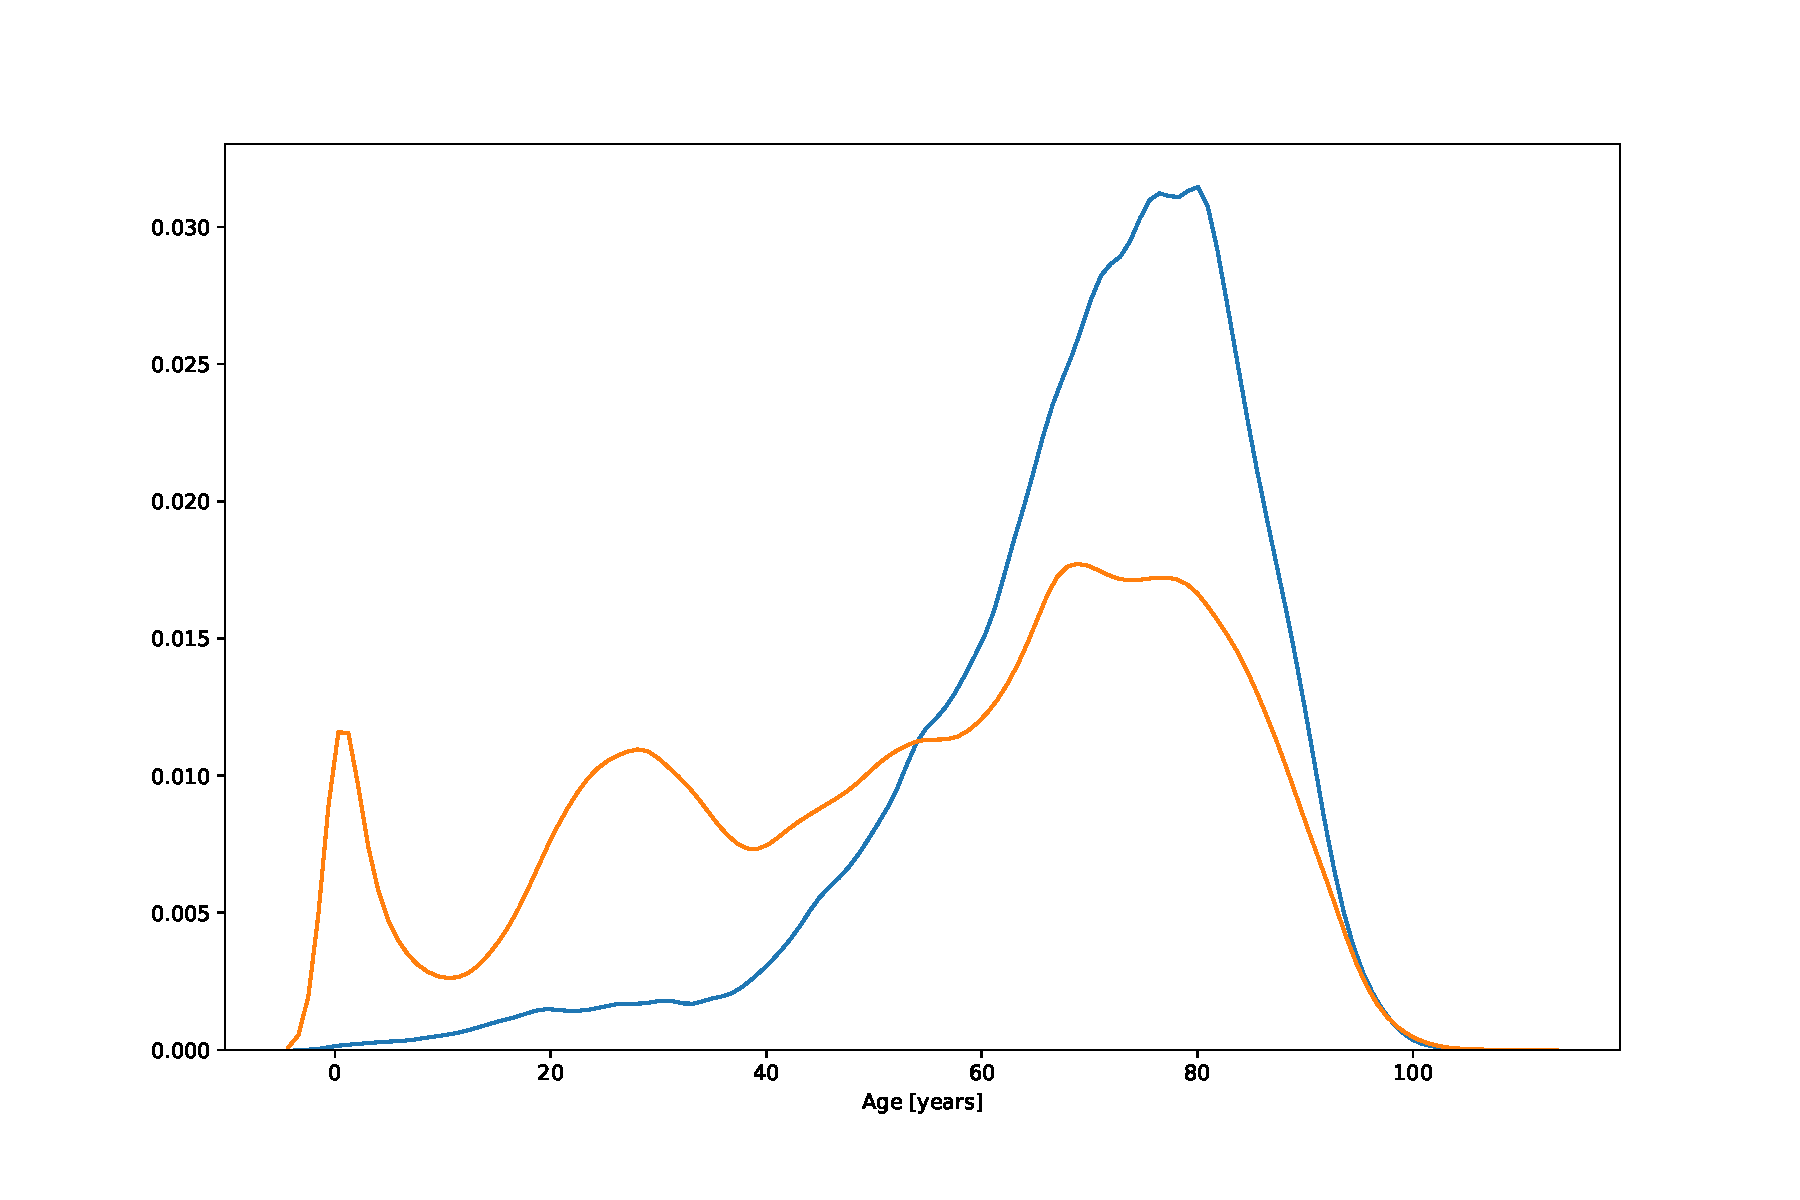
\includegraphics[width=\linewidth]{img/Diabetes-Age-kde.pdf}
    \captionof{figure}{Estimated p.d.f. for age (years) split as in
        Fig~\ref{fig:diabetes-LOS-kde-plot}}
    \label{fig:diabetes-Age-kde-plot}
    \end{minipage}
\end{figure}


\subsection{Ward}\label{subsec:ward}

Are the results from the paper reproducible with our data?


%\printbibliography
\end{document}
